\section{Results and Discussion}

We present results with different types of flow field data sets to evaluate our approach, including synthetic data and spatially aggregated data sets. To demonstrate the effectiveness of the proposed algorithm, we compared it with the Monte Carlo (MC) method, which is the general approach to stochastically trace particles in uncertain flow fields. We performed quantitative comparisons on the resulting streamlines generated by our approach and the MC method with different settings and distance measurements. We also qualitatively compare the most likely streamlines as well as the distributions of possible traces produced by our approach and the MC method by visualizing sample traces on different data sets.

\subsection{Synthetic Data}

We first evaluate the proposed algorithm on the analytical static double-gyre data set proposed by Shadden et al. in~\cite{Shadden2005271}. Gaussian noise is added into the vector field to synthesize the uncertainty. In order to quantitatively evaluate the robustness of the proposed algorithm under the influence of noise, we generate streamlines starting from regularly sampled seed positions for the certain double-gyre data set and use those streamlines as our ground truth. Then, a set of sample traces are generated by the MC method and the Bayesian approach starting from the same seed position presented above for the uncertain double-gyre data set with different noise level, which is controlled by the standard deviation $\sigma$ of the Gaussian noise. All the streamlines were generated with a step size of $0.005$ and a maximum step number of $100$. For the Monte Carlo method and the proposed algorithm, a critical parameter is the number of particles used for each seed. Indeed, more particles will give a more accurate presentation of the target distribution but will take more time to generate the results. Hence, a particle count that balances the accuracy and the computation time need to be studied. Based on~\cite{journals/mia/PontabryROSKD13}, we use $100$ particles for both of the methods in the experiments. To compare the accuracy of the resulting traces, the Hausdorff distance~\cite{Roessl:2012:TVCG} and the Mean of the closest point distance~\cite{Corouge04towardsa} between streamlines were used. Figure~\ref{gerror} gives the average of the distances presented above between the most likely streamlines generated from each method and the ground truth, with increasing $\sigma$ values for the noise in the vector field. The figure reveals that our method can produce most likely traces that are closer to the ground truth and the average of the distances increases more slowly than the MC method as the noise increases.

Besides comparing the accuracy of the most likely traces, it is also important to compare the whole distribution of possible traces generated by each method. We evaluate the accuracy of uncertain streamlines starting from a given seed position by measuring the distance between each individual trace and the ground truth, then we compute the weighted sum of all the distances. For the MC method, all traces are equally weighted. For the proposed method, the weights of the traces described above are used. Figure~\ref{gerror_r} shows that the proposed method can generate more accurate traces with less uncertainty.

\begin{figure}[!htb]
  \centering
  \begin{subfigure}[b]{0.24\textwidth}
    \centering
    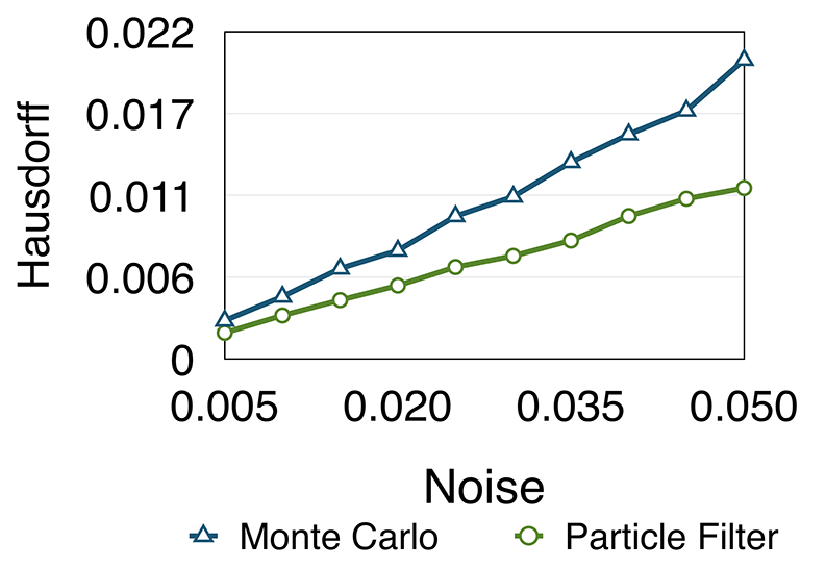
\includegraphics[height=0.8in]{../figures/doublegyre_h.eps}
  \end{subfigure}~
  \begin{subfigure}[b]{0.24\textwidth}
    \centering
    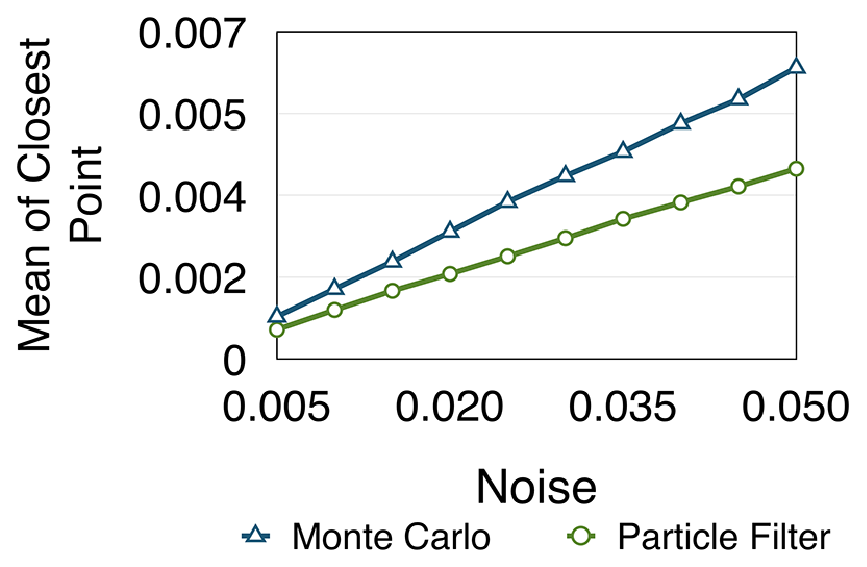
\includegraphics[height=0.8in]{../figures/doublegyre_m.eps}
  \end{subfigure}
  \caption{Comparison of the distance between the most likely traces and the ground truth for our method and the MC method.}
  \label{gerror}
\end{figure}

\begin{figure}[!htb]
  \centering
  \begin{subfigure}[b]{0.24\textwidth}
    \centering
    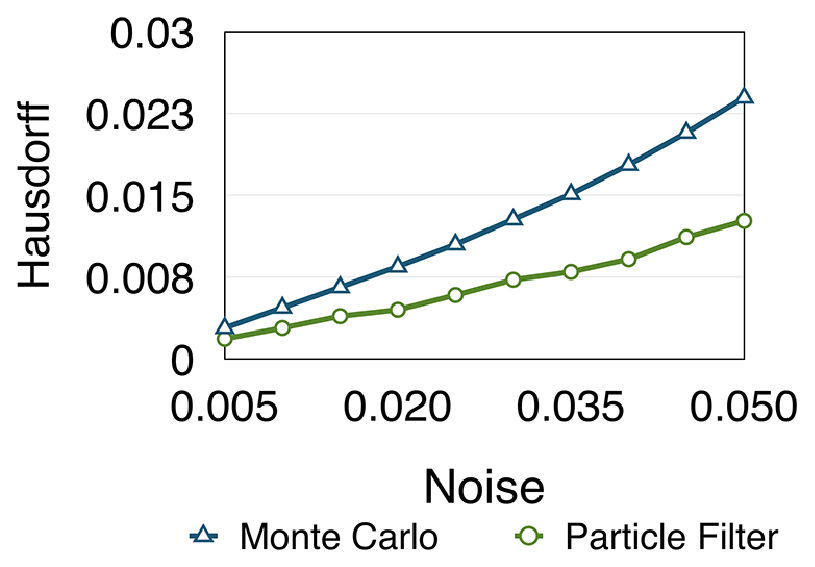
\includegraphics[height=0.8in]{../figures/doublegyre_hr.eps}
  \end{subfigure}~
  \begin{subfigure}[b]{0.24\textwidth}
    \centering
    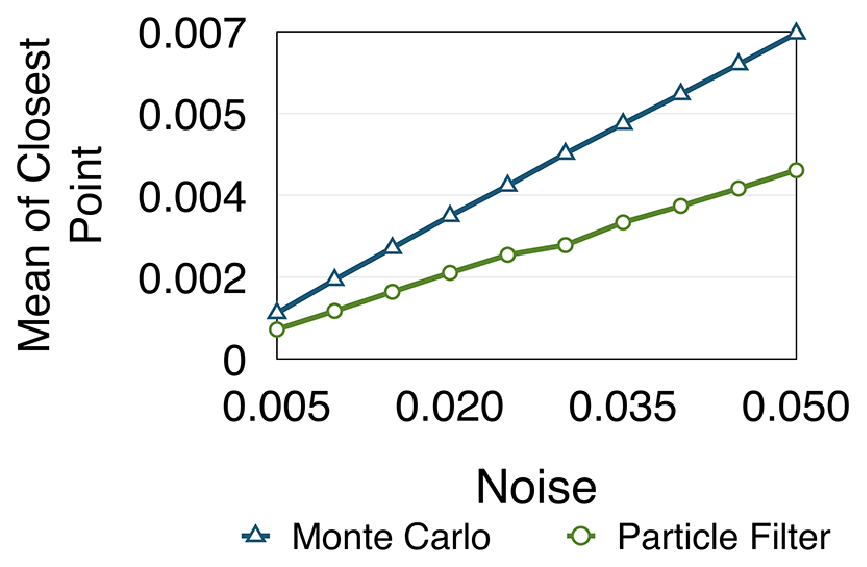
\includegraphics[height=0.8in]{../figures/doublegyre_mr.eps}
  \end{subfigure}
  \caption{Comparison of overall trace accuracy. For each method, distances of all sample traces to the ground truth are measured and summed by their weights.}
  \label{gerror_r}
\end{figure}

Figure~\ref{case_1} shows sample traces generated by the MC method and the proposed method at a given seed location in the double-gyre flow field. As we can see in the figure, our method can generate more concentrated traces which are also closer to the ground truth compared with the MC method. The most likely trace generated by the proposed method is also closer to the ground truth, as shown in~\ref{case_1} (c).

\begin{figure}[!htb]
   \centering
  \small
  (a) \vcenterbox{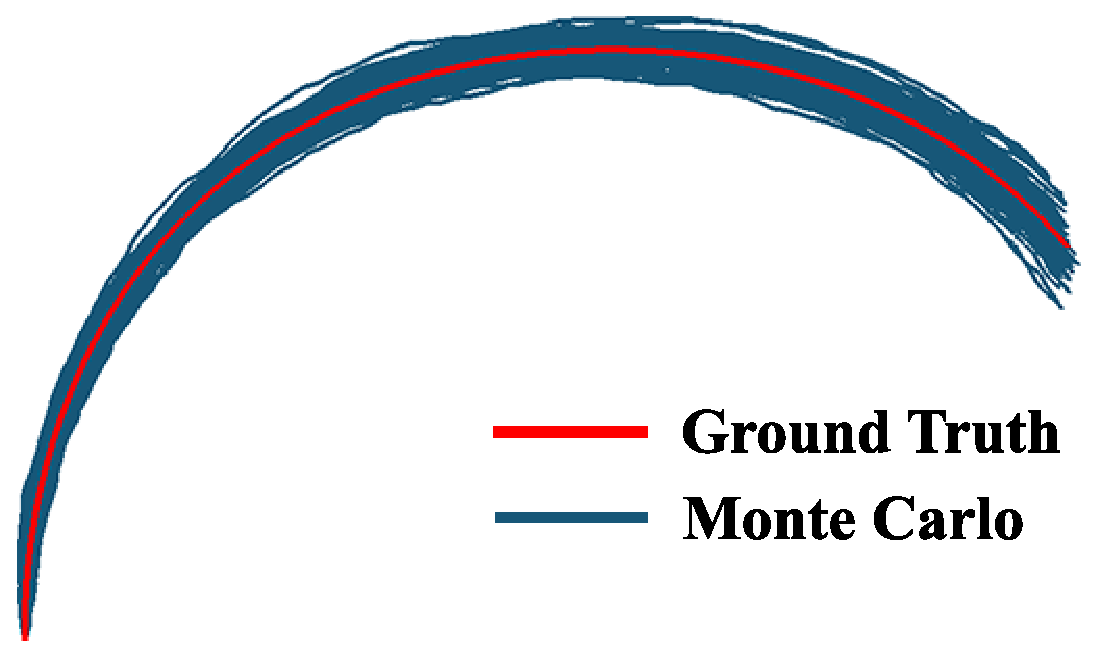
\includegraphics[height=0.5in]{../figures/double_gyre_mc35.eps} } \hfill
  (b) \vcenterbox{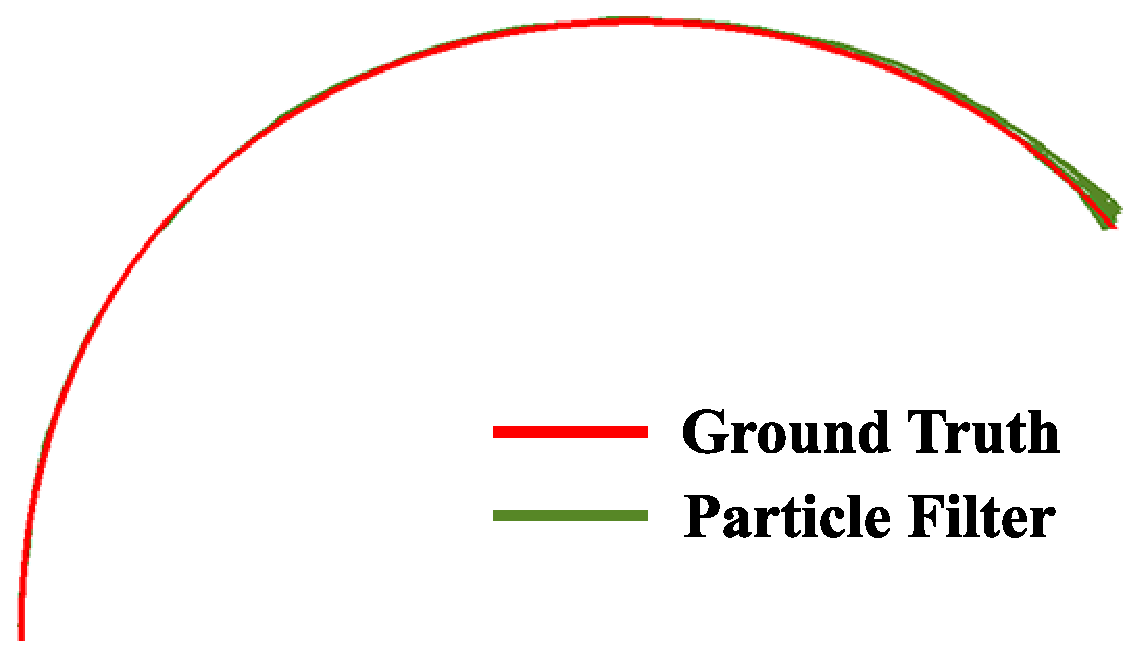
\includegraphics[height=0.5in]{../figures/double_gyre_smc35.eps} } \hfill
  (c) \vcenterbox{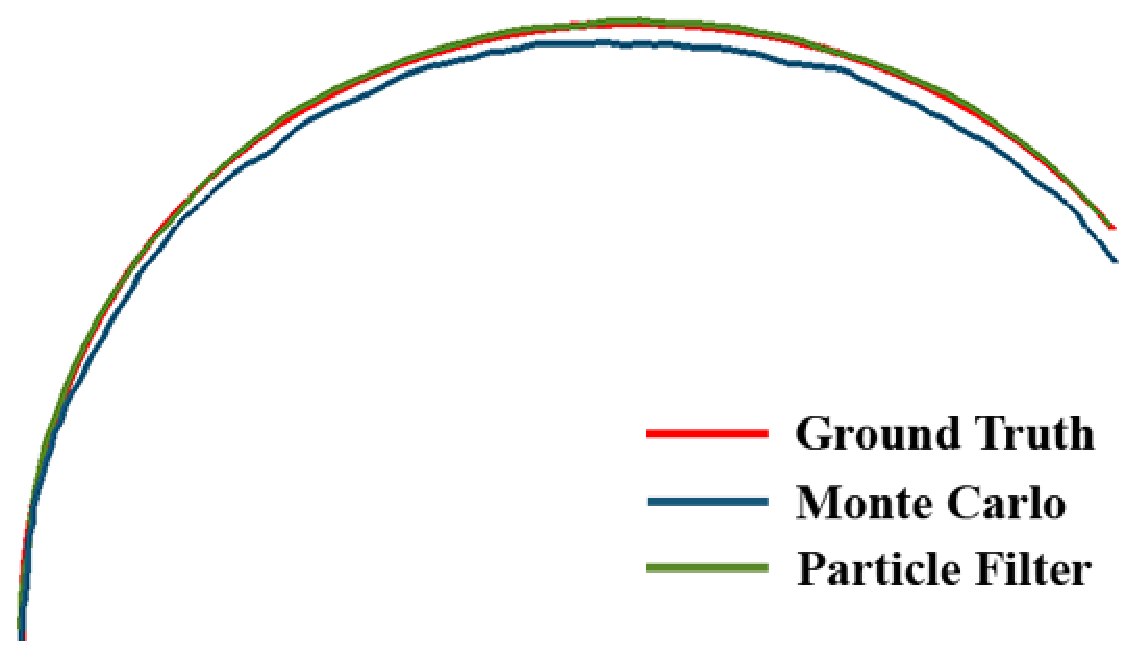
\includegraphics[height=0.5in]{../figures/double_gyre_opt35.eps} }
  \caption{(a): Sampled streamlines computed by the MC method starting from seeding position $x=0.3, y=0.5$ in the analytical double-gyre data set. (b): Sampled streamlines computed by our method from the same seeding position in (a). (c): The most likely traces generated by both methods compared with the ground truth.}
  \label{case_1}
\end{figure}

\subsection{Spatially aggregated Data Sets}

\begin{figure*}[!htbp]
  \centering
  \small
  (a) \vcenterbox{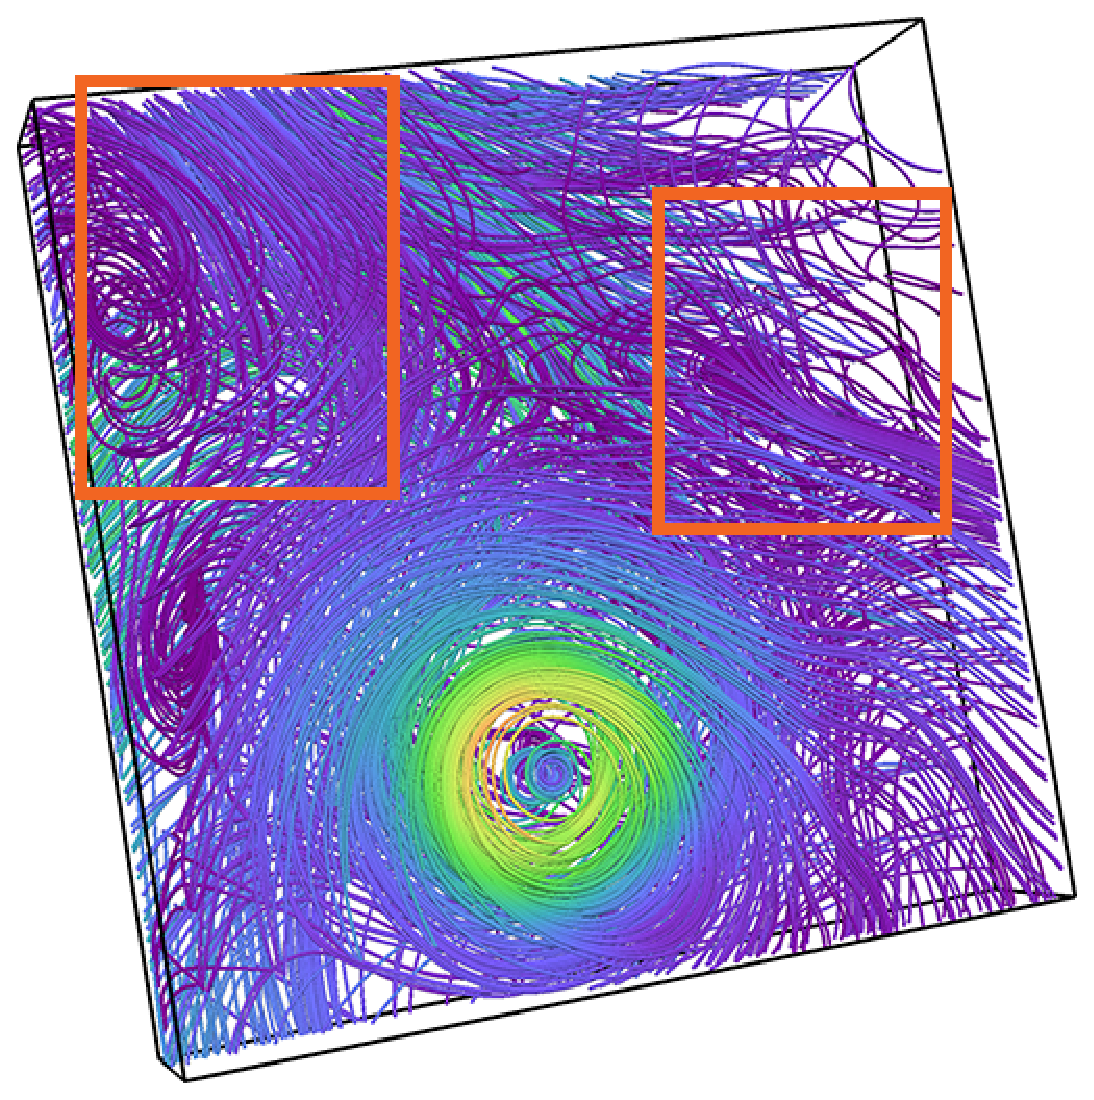
\includegraphics[width=1.5in]{../figures/isabel_gt.eps} } \hfill
  (b) \vcenterbox{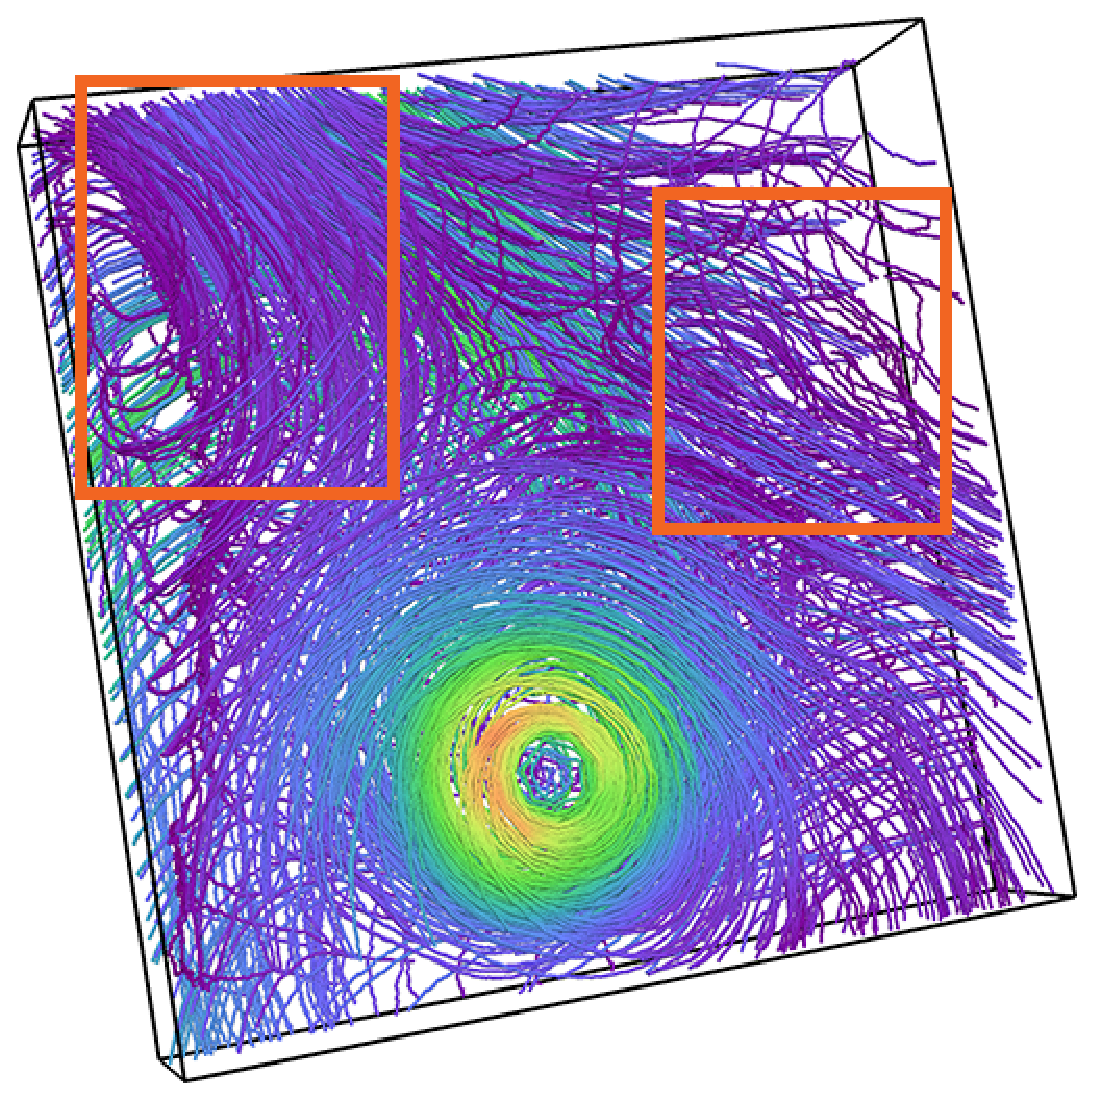
\includegraphics[width=1.5in]{../figures/isabel_mc.eps} } \hfill
  (c) \vcenterbox{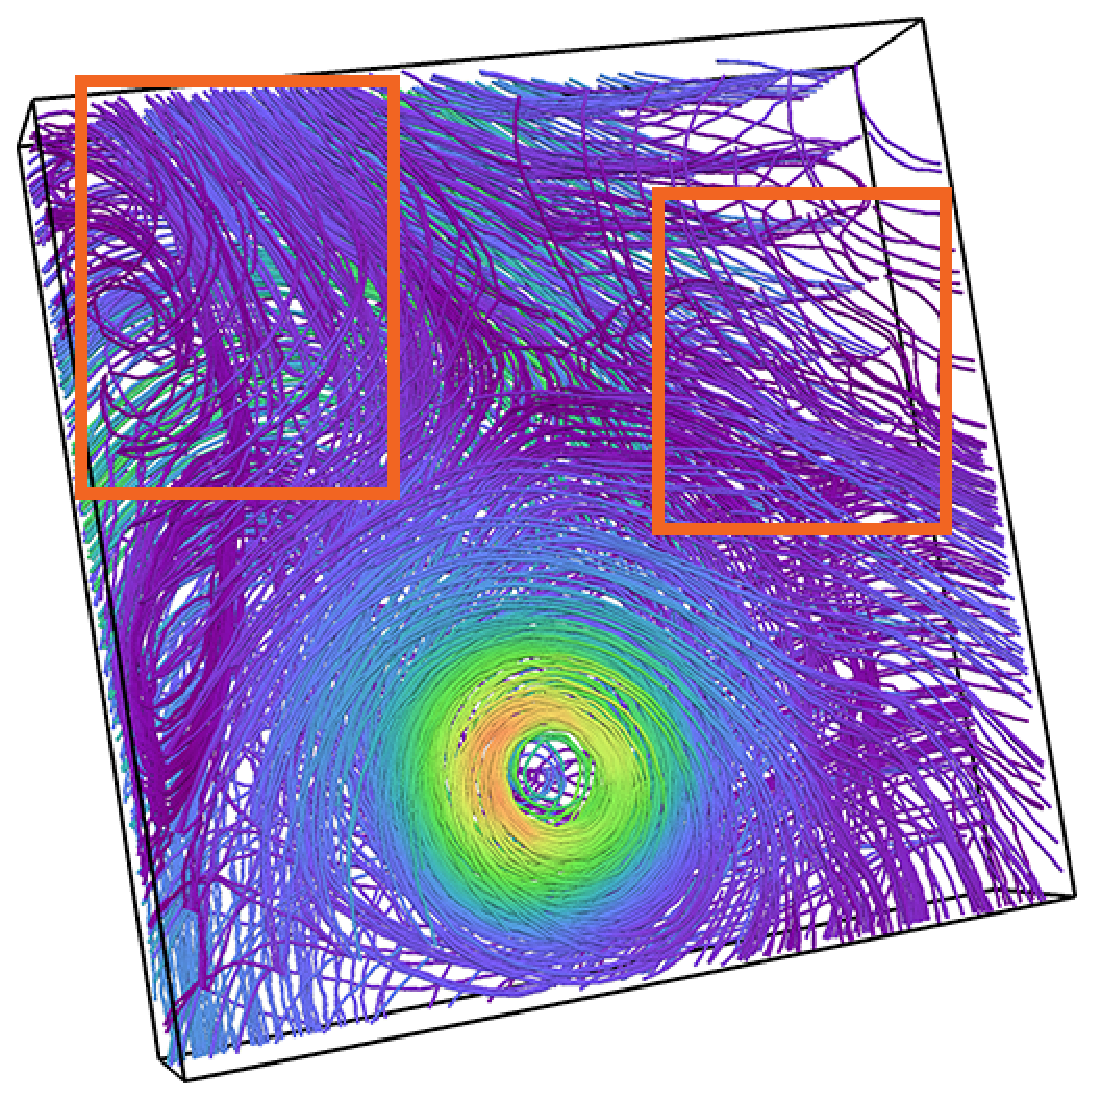
\includegraphics[width=1.5in]{../figures/isabel_smc.eps} }

  \caption{Streamlines generated on the Hurricane Isabel data sets. The color is used to enhance the contrast among streamlines. (a): The ground truth streamlines generated on the raw data. (b): Results produced by the Monte Carlo method on the distribution data with block size $16^3$. (c): Streamlines generated by our method on the same data in (b).}
  \label{data_overview}
\end{figure*}

\begin{figure}[!htbp]
  \centering
  \small
  (a) \vcenterbox{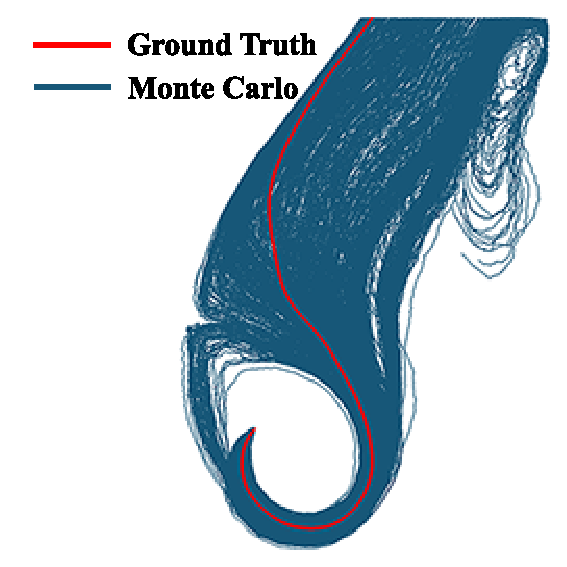
\includegraphics[height=1.0in]{../figures/isabel_mc1.eps} } \hfill
  (b) \vcenterbox{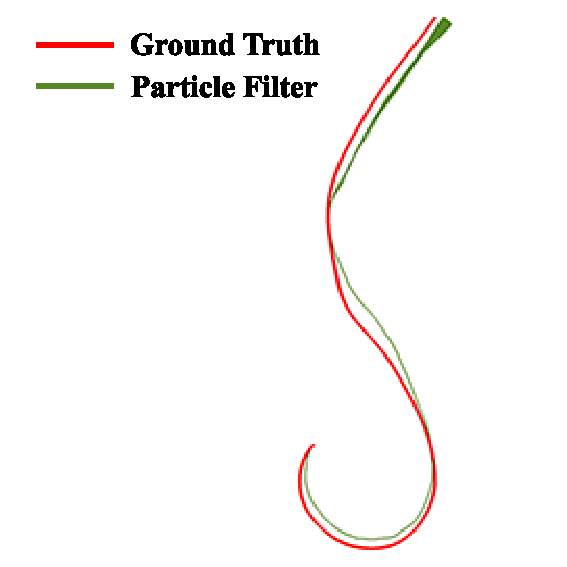
\includegraphics[height=1.0in]{../figures/isabel_smc1.eps} }
  \caption{(a): Sampled streamlines computed by the MC method starting from seeding position $x=250, y=150, z=45$ in the Isabel data set. (b): Sampled streamlines computed by our method from the same seeding position in (a).}
  \label{case_4}
\end{figure}

In this section, experiments were done on the Hurricane Isabel data set. Hurricane Isabel is a data set with a resolution of $500 \times 500 \times 100$ that models a strong hurricane in the west Atlantic region in September 2003. In order to test the performance of our algorithm on uncertain data which represented by non-gaussian distributions, we decompose the data into small cubic blocks and construct a histogram for each block. For the test data set, distribution-based data are generated with three different block size $8^3$, $16^3$, and $32^3$ to evaluate the performance of the proposed algorithm under the influence of uncertainty.

As presented above, we regularly sample a set of seed locations and compute the streamlines for both the raw data and the spatially down sampled data. To perform the quantitative analysis, we treat the streamlines computed from the raw data as the ground truth and compute the distance between the stochastic particle traces with the ground truth. $100$ particles were used with a integration step size $1.0$ and a maximum step number of $1000$ for the streamline computation. Figure~\ref{berror_r} gives the mean of the distances' weighted sum between sample streamline bundles generated from the test methods and the ground truth on the test data set with different block sizes. The figure reveals that the proposed method can produce traces that are closer to the ground truth.

\begin{figure}[!htb]
  \centering
  \begin{subfigure}[b]{0.24\textwidth}
    \centering
    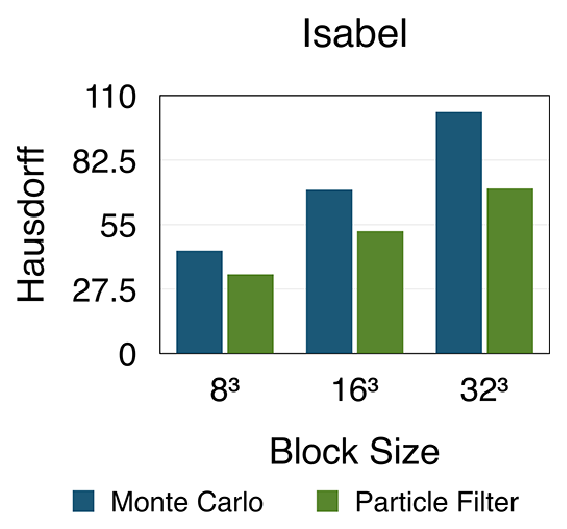
\includegraphics[height=0.9in]{../figures/isabel_h.eps}
  \end{subfigure}~
  \begin{subfigure}[b]{0.24\textwidth}
    \centering
    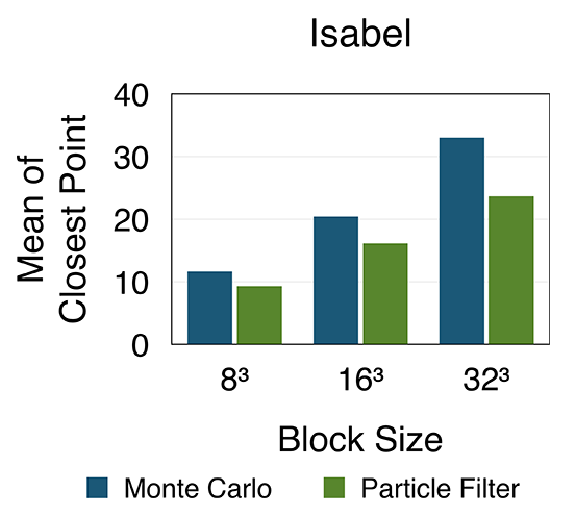
\includegraphics[height=0.9in]{../figures/isabel_m.eps}
  \end{subfigure}
  \caption{Distances between the ground truth and sample traces generated by our method and the MC method for the Isabel data set.}
  \label{berror_r}
\end{figure}

Figure~\ref{data_overview} shows the streamlines generated from the test data set on the seed positions presented above. The most likely streamlines generated by the MC method on the distribution-based data set with block size $16^3$ are given in Figure~\ref{data_overview} (b); as expected, streamlines generated by the MC method are generally not as smooth as the ground truth and some flow features looks quiet different compare with the ground truth. Figure~\ref{data_overview} (c) show the streamlines produced by our method with the same block size, which give more accurate and smoother results. Figure~\ref{case_4} gives sample traces generated by the MC method and the proposed method at a given seed location in the Isabel data set. Figure~\ref{case_4} shows that our algorithm can produce more concentrated and accurate results than the basic MC method, because the correlation between consecutive integration steps are exploited.

\subsection{Performance}

All the experiments were performed on a desktop computer with an Intel(R) Core(TM) i7-4790K CPU 4.0GHz processor, 16GB memory, and an NVIDIA GTX 970 GPU. In Table~\ref{timing}, we compare the performance measurements between the proposed algorithm and the Monte Carlo method for streamlines estimated for a given seed position with $100$ sample points for all the test data sets used in this paper. In all the datasets, our approach is almost as fast as the Monte Carlo method.

\begin{table}[!htb]
\centering
\begin{tabular}{|c|c|c|c|c|}
\hline
\multirow{2}{*}{Data Set}    & \multirow{2}{*}{Method}     & \multicolumn{3}{c|}{Timing(sec)}  \\ \cline{3-5}
                             &                             & 40 Steps  & 80 Steps & 120 Steps  \\ \hline
\multirow{2}{*}{Double Gyre} & MC                          & 0.0026    & 0.005    & 0.008      \\ \cline{2-5}
                             & Bayesian             & 0.0035    & 0.007    & 0.01       \\ \hline
\multirow{2}{*}{Isabel}      & MC                          & 3.3       & 6.7      & 10.1       \\ \cline{2-5}
                             & Bayesian             & 3.4       & 6.8      & 10.7       \\ \hline

\end{tabular}
\caption{Overview of the performance for the proposed algorithm and the Monte Carlo method.}
\label{timing}
\end{table}
